%!TEX root = chapter-experiment.tex
\section{Genuine and Impostor Distributions}
\label{sec:experiment:distribution}

Figure ~\ref{fig:experiment:11p} show the genuine and impostor distributions when the 15-dimensional features are applied to the 4000 training database when calculate the Euclidian distance.

\begin{figure}[htb]
  \begin{center}
    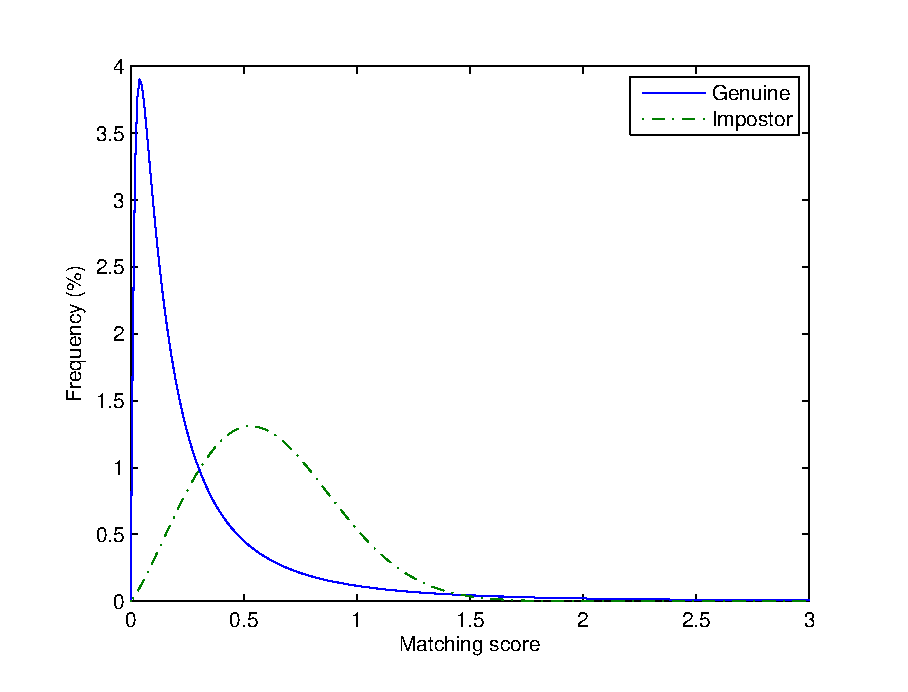
\includegraphics[scale=1]{ch-experiment/figures/11p.eps}
    \caption[Sample distribution by matching score]{Sample distributions by matching the 15-dimensional feature vector}
    \label{fig:experiment:11p}
  \end{center}
\end{figure}

